\documentclass[11pt]{article}

\usepackage[margin=0.7in]{geometry}
\usepackage{changepage}
\usepackage{hyperref}
\usepackage{graphicx}
\usepackage{amsmath}
\usepackage{xcolor}
\usepackage{xparse}

\def\labelitemi{\ensuremath{\triangleright}}
\renewcommand{\url}[1]{{\texttt{#1}}}
\renewcommand{\line}[2]{{\vspace{12pt} \large \noindent\textbf{\textsc{#1}} \hfill \small{#2}}{\vspace{2pt}\hrule\vspace{4pt}}}

\newif\ifisleft
% \isleftfalse % by default

%%% Get an environment variable from latex. %%%
% Shamelessly stolen from 
% https://tex.stackexchange.com/questions/62010/can-i-access-system-environment-variables-from-latex-for-instance-home
\ExplSyntaxOn

\NewDocumentCommand{\getenv}{om}
{
\sys_get_shell:nnN { kpsewhich ~ --var-value ~ #2 } { } \l_tmpa_tl
\tl_trim_spaces:N \l_tmpa_tl
\IfNoValueTF { #1 }
  {
  \tl_use:N \l_tmpa_tl
  }
  {
  \tl_set_eq:NN #1 \l_tmpa_tl
  }
}

\NewDocumentCommand{\strcmp}{mmmm}{
  \str_if_eq:eeTF{#1}{#2}
    { #3 }
    { #4 }
}

\ExplSyntaxOff

\begin{document}

  \setlength{\parindent}{0em}
  \pagestyle{empty}

  \getenv[\withpic]{WITHPIC}
  
  \noindent\begin{minipage}{0.64\textwidth}
    
    {\LARGE{\textbf{Jacopo Philip Moretti}}}

    \vspace{0.5em}
    \textit{CS MSc student at EPFL, with interests in theorem provers, formal verification, and languages, both natural and programming.}

    \vspace{0.5em}
    {
      \small
      \href{https://github.com/quartztz}{\url{github.com/quartztz}} :: \url{+41 76 730 67 19} :: \url{jacopo @ }\href{https://quartztz.com}{\url{quartztz.com}}
    }
  \end{minipage}
  \strcmp{\withpic}{true}{
    \begin{minipage}{0.25\textwidth}
      \begin{center}
        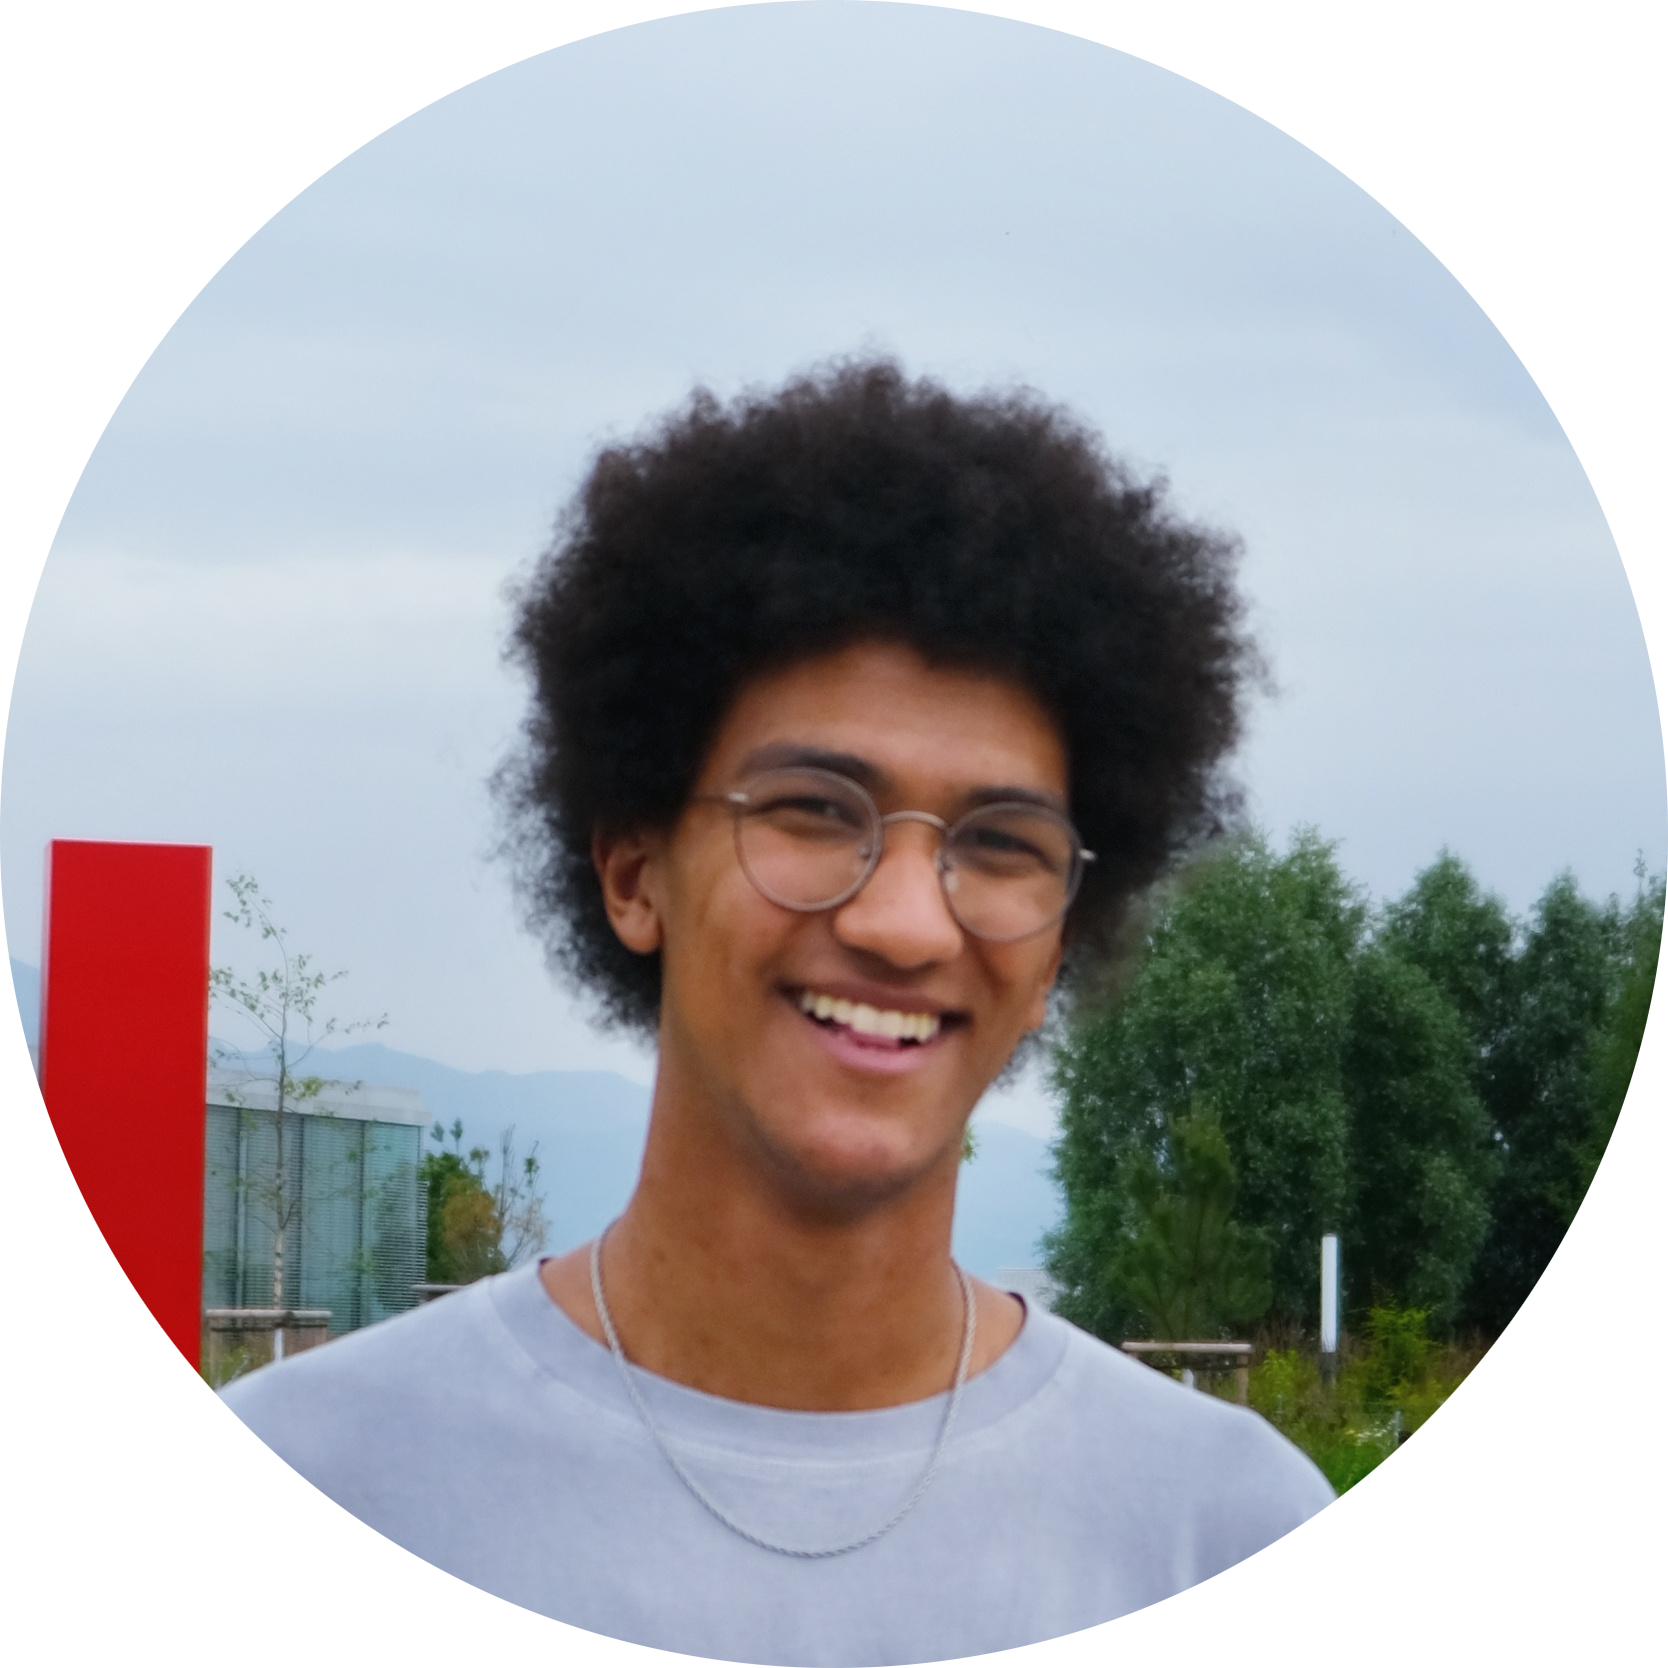
\includegraphics[width=.75\textwidth]{"./assets/img_circ.png"}
      \end{center}
    \end{minipage}
  }{
    % empty
  }

  \section*{Academic}
  \vspace{-1.5em}

  \line{MSc in Computer Science :: EPFL}{2024 - \textsc{Present}}

  Master's Degree in Computer Science at EPFL, \textit{Foundations of Software} specialization.

  \textbf{Projects:} Verified WebAssembly Decompilation, Lean formalization of theoretical CompSci result.

  \textbf{Fields of interest:} Theorem Proving, Software/Hardware Verification, Programming Languages.

  \textbf{Relevant courses:} \textit{Interactive Theorem Proving, Foundations of Software, Algorithms II, Formal Verification}.

  \line{BSc in Computer Science :: EPFL}{2021 - 2024}

  Bachelor's degree in Computer Science from EPFL.

  \textbf{Fields of interest:} Functional Programming, Programming Languages.

  \textbf{Relevant courses:} \textit{Functional Programming, Computer Language Processing, Mathematical Logic}.

  \section*{Experience}
  \vspace{-1.5em}

  \line{Chief Product Officer :: Actualia}{2024 - \textsc{Present}}

  CPO at \textit{actualia}, a startup building an AI-powered pipeline to deliver relevant and verifiable press reviews. 
  Managed design team and led frontend development, raised 12k CHF in grants.

  \line{Teaching Assistant :: EPFL}{2023 - \textsc{Present}}

  Teaching assistant for various courses at EPFL. Assisted students on forums and in-person.

  \vspace{-0.5em}
  \begin{itemize}
    \item \textit{Formal Verification (Kuncak, F25)}: assist exercise set and lab design, VSCode extension for \href{https://github.com/epfl-lara/stainless}{\url{Stainless}}.
    \item \textit{Computer Language Processing (Kuncak, S25)}: assisted with exercise set design and grading.
    \item \textit{Software Construction (Kuncak, Odersky, Pit-Claudel, F23)}: (Fall 2023) implemented workflow for recording and editing 20+ video lectures per day.
  \end{itemize}
  \vspace{-1em}

  \line{Technical Manager :: Fréquence Banane}{2022 - 2024}

  Committee member tasked with maintaining the technical (audiovisual and server) infrastructure of an 80+ member student radio. Gained knowledge in writing code for large scale and long term use, managing a technical team, and audio engineering.

  \section*{Skills}

  \vspace{-0.5em}
  \begin{adjustwidth}{6em}{}
    \begin{itemize}
      \item[\textbf{Languages}] Italian (native), French (native), English (fluent), German (basic).
      \item[\textbf{Programming}] Rocq/Coq, Scala, Lean, Typescript, Rust, Dart, Python, React, Vue, Java, C.
      \item[\textbf{Tools}] Git, Docker, Proxmox, Typst, LaTeX, Markdown
      \item[\textbf{Design}] Adobe Suite, Figma, Penpot.
      \item[\textbf{Other}] Audio Engineering, Video Editing, Stagecraft.
    \end{itemize}
  \end{adjustwidth}

\end{document}
